\subsection{Architecture des applications}
\label{sec:3}
Les applications destinées aux tables interactives sont des SI conçus suivant un modèle d'architecture. Pour Nigay, les modèles d'architectures préconisent une séparation entre les services du Noyau Fonctionnel (NF) et ceux de l'Interface Utilisateur (UI) , et définit une stratégie de répartition des services de l'interface qui se traduit par un ensemble de constituants logiciels [Nigay 1994].  Dans cette section nous présentons quelques modèles architectures.
\subsubsection{Modèle de Seeheim}
Le modèle de Seeheim [Pfaff 1985] est l'un des premier modèle d'architecture qui préconise l' éclatement du SI en trois composants distincts (cf. figure \ref{fig:7}). Le composant Application Interface Model décrit la sémantique de l'application du point de vue utilisateur, il est composé de structures de données et de fonctionnalités. Le composant Presentation définit la manière avec la quelle le système peut être manipulé par l'utilisateur en entrée ou en sortie. Son niveau d'abstraction est lexical pour l'utilisateur, car il est décrit à l'aide des composants graphiques et des langages d'interactions. Le composant Dialogue Control gère la communication entre ces deux composants.
\begin{figure}[ht]
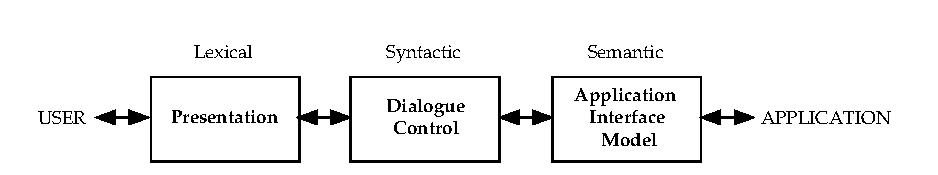
\includegraphics[width=432pt]{chap2/img-8.eps}
%
\includegraphics[width=432pt]{chap2/img-6.eps}
\caption{Trois composants d'UI du modèle de Seeheim}\label{fig:7}
\end{figure}
\subsubsection{ARCH}
ARCH [UIMS 1992] est un modèle d'architecture qui se base sur des composants conceptuels du modèle de Seeheim [Pfaff 1985]. Comme l'indique la Figure 2 5, ce modèle permet une séparation entre le NF, le Contrôleur de Dialogue (CD) et la Présentation. Les deux pieds de l'arche sont des composants spécifiques à une plateforme; le composant NF décrit un domaine précis et les composants d'Interaction sont liés à des dispositifs du monde réel. Le CD gère l'enchainement des tâches ainsi que les liens avec les objets des deux composants voisins. L'Adaptateur de domaine joue un rôle d'interface avec le composant NF pour corriger les différences de conceptions. Le composant Présentation est une boîte à outils virtuelle, telle que XVT [Valdès 1989] qui implémente les objets de présentations concrétisés en fin de compte par les objets d'interaction de la bibliothèques graphiques.
PAC-Amodeus [Nigay 1994] est un modèle d'architecture basé sur ARCH, il permet de définir plusieurs contrôleurs de dialogue pour une application grâce aux agents  PAC.  
\begin{figure}[ht]
\begin{center}
\includegraphics[width=340pt]{chap2/img-7.eps}
\caption{Composants du modèle ARCH}\label{fig:5}
\end{center}
\end{figure}
\subsubsection{MVC}
MVC [Krasner and Pope 1988] est un modèle d'architecture pour la conception des systèmes interactifs réutilisables. Il divise les applications en trois types de composants : le modèle, la vue et le contrôleur. Le modèle est une représentation du domaine d'une application, il peut contenir des données, des services, etc., il fait partie du NF d'une application. La vue est la structure de l'UI d'une application, elle est constituée des éléments d'une boîte à outils qui permettent de décrire une présentation. Le contrôleur est une interface entre le modèle, la vue et les dispositifs d'interactions en entrée.
En considérant une partie de l'UI de l'application CBA, la figure \ref{fig:6} est une instance des différents éléments du modèle MVC. La Vue est composée de JPanel, JLabel, JComboBox et d'une JList contenant des images. La sélection d'une catégorie du sélecteur JComboBox  avec un clavier ou une souris modifie la liste d'images en faisant d'abord appel au contrôleur de JComboBox ensuite au modèle de JList pour mettre à jour la vue.
La migration de cet artéfact d'UI vers une table interactive qui supporte la bibliothèque graphique DiamondSpin par exemple implique la modification de la vue en remplaçant les composants graphiques par leurs équivalents et en adaptant le code du contrôleur et du modèle pour remplacer les variables correspondant aux composants graphiques de la vue. Par exemple dans le cas o\`{u} DSComboBox correspond à JComboBox dans DiamondSpin, le type de la variable cb du contr\^{o}leur doit \^{e}tre remplacé dans le contr\^{o}leur et le mod\`{e}le.
Par conséquent, la migration de l'UI vers la table interactive avec cette hiérarchie implique une modification à la fois du contr\^{o}leur, de la vue et du mod\`{e}le. Pour éviter ces modifications, il faut que le code des applications à migrer respecte des heuristiques qui favorisent la réutilisation des différents composants de l'application. Parmi ces heuristiques on peut citer: la séparation entre les éléments spécifiques à la plateforme (PSM) et les éléments indépendants de la plateforme (PIM) au niveau du contr\^{o}leur et de la vue d'une part, et la non utilisation des éléments PSM du contrôleur de la vue au niveau du modèle d'autre part. Cette séparation permettra de changer les contr\^{o}leur de dialogue spécifiques aux dispositifs d'interaction et les vues spécifiques aux biblioth\`{e}ques graphiques.
\begin{figure}[ht]
\begin{center}
\includegraphics[width=432pt]{chap2/img-2.eps}
\caption{Modèle Vue Contrôleur}\label{fig:6}
\end{center}
\end{figure}
\subsubsection{Résumé}
Nous avons présenté dans cette section le modèle d'architecture de Seeheim qui préconise une séparation entre le composant d'application et le composant de présentation avec un composant contrôleur de dialogue, mais le composant de contrôleur de dialogue de ce modèle est fortement lié au composant de présentation et au composant d'application et un changement du composant de présentation par exemple implique aussi l'adaptation du contrôleur de dialogue. Le modèle ARCH est conçu pour résoudre cette limitation du modèle de Seeheim, il préconise l'utilisation d'un composant de présentation qui décrit de manière abstraite et indépendamment d'une plateforme les éléments de l'UI et sert de mapping entre le contrôleur de dialogue et les composants d'interactions. Un changement de la présentation n'impactera pas le contrôleur de dialogue mais le mapping entre ces deux modèles. Les modèle d'architecture PAC et MVC quand à eux sont à base d'agent qui permet de décrire des interfaces permettant les manipulations directes [Crease 2001]. MVC par exemple permet une séparation entre les interactions entrée décrites au niveau des contrôleurs et les interactions sortie. Cette séparation facilite le changement des interactions en entrée. Nous avons aussi présenté dans cette section la nécessité de décrire pour l'architecture MVC des contrôleurs et des vues ayant deux niveaux d'abstraction.
